\documentclass[english]{proposalnsf}
\usepackage{graphicx}
\usepackage{url}
\usepackage[square,numbers]{natbib}
\usepackage[nottoc,numbib]{tocbibind}

\title{My Awesome TechReport}
\author{Philip Johnson \\Collaborative Software Development Laboratory \\ Information and Computer Sciences \\ University of Hawaii}

\begin{document}
\maketitle
\tableofcontents
\newpage

\section{Introduction}
\label{introduction}

The introduction section typically begins with a description of a {\em Big Problem}.  For example, ``Computer science has a problem with diversity.  The percentage of women in computer science has actually dropped by almost half since the 1980's'' \cite{camp_generation_2017}.  A Big Problem is typically a problem that is way too big for your research project to actually solve by itself. The description of the big problem is typically a few paragraphs to a page in length, and should have some citations to research establishing the Big Problem as a big problem.

The next part of the introduction section presents the {\em Small Problem}--- the problem that you are actually going to attempt to address in your research project, and how it relates to the Big Problem.  For example, ``In order to understand how to increase representation of women in computer science, we must first begin to understand why women might start a computer science degree program but not finish it. In this research project, I will investigate what students believe to be barriers to completing a computer science degree, and whether or not women perceive these barriers differently.''  The description of your Small Problem should also be a few paragraphs to a page in length.

The final part of the introduction section describes how the rest of this document is organized, which should also lead the reader through your research process.  For example, ``Section \ref{related-work} discusses research related to gender in STEM disciplines including computer science.  Section \ref{research-design} presents the research process I will use in order to gather data related to barriers to completion of a computer science degree program.  Section \ref{results} presents the data I will collect and how I will analyze it.  Section \ref{conclusions} presents my conclusions and proposals for future research.''

\section{Related Work}
\label{related-work}

The Related Work section presents research and/or technology that you are using as a basis for your project.  Related Work sections generally should establish the following:

\begin{itemize}
\item Your research project is novel---no one else has already definitively solved your Small Problem.
\item Your research project is important. You can discuss research that provides more detail about the Big Problem, for example. This might include research on the economic or social costs of the Big Problem.
\item Your research project is important.  Another way to show importance is to discuss research by other people related to your Small Problem, but that doesn't provide all of the insight your project will provide.
\item The technologies you plan to use, or technologies related to what you are going to do. If your project involves technology implementation, then you will want to talk about related technologies in this section.
\end{itemize}

\section{Research Design}
\label{research-design}

This section describes how you intend to go about addressing your Small Problem.  If you need to implement some technology, you can provide a specification (perhaps with mockup screens) for what you are going to implement. If you are going to do a survey or collect data in some way, you should describe what data you are going to collect.

If you are doing a survey, then this section should include the {\em instruments}:  for example, what questions, specifically, do you intend to ask?

You want this section to be as detailed as you can possibly make it.  The more detail, the easier it is for your colleagues to critique and find opportunities for improvement.   It's way harder to make changes after you've already done the implementation or conducted the interviews or whatever!

Sometimes you might do a {\em pilot study} or {\em spike solution}.  This is a quick and dirty implementation that helps you understand the nature of the problem you are trying to solve.  For example, you might interview a single person, or you might make a mockup implementation or analysis with fake data.  That's fine: include the results of this section.

Quite often, you will want to add a picture to your tech report. The trick for including figures into LaTeX is to first convert them to encapsulated postscript (.eps) format. I use the convert program, but for Windows, you might ned pdftoops or ghostscript.  Google for lots of ideas on how to do this. All figures in your tech report must be referenced. So for example, Figure \ref{fig:theory} presents a theory of change for the RadGrad project.

\begin{figure}[t]
  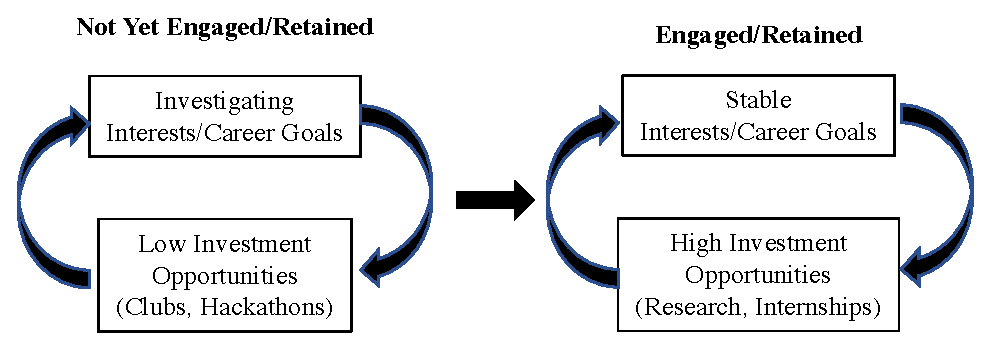
\includegraphics[width=\textwidth]{theory-of-change.eps}
  \caption{Theory of change}
  \label{fig:theory}
\end{figure}

You might also want to include a table.  Figure \ref{fig:hardware-table} shows an example table.

\begin{figure}[ht]
  \begin{tabular}{l|r|p{2in}|p{1in}|p{1in}} \hline
  {\bf Device} & {\bf Cost} & {\bf Measurements} & {\bf Synchronization} & {\bf Communication} \\ \hline
  PMU & \$100,000 & frequency, voltage, current & GPS & Secure LAN  \\
  FDR & \$2,500 & frequency, voltage & GPS & Internet \\
  PQube & \$5,000+ & frequency, voltage, THD, VARs & (none) & (none)  \\
  mPMU & \$5,000+ & frequency, voltage, THD, VARs & GPS & Custom network \\
  AC Scout & \$200+  & frequency, voltage & (none) & (none) \\
  OPQ & \$60 & frequency, voltage, THD & NTP & HTTP/SSE \\
  \hline
  \end{tabular}
  \caption{Comparison of hardware devices for power quality monitoring}
  \label{fig:hardware-table}
\end{figure}


\section{Results}
\label{results}

This section is not needed in a tech report intended as a proposal.  Once you have completed your project, then you can add this section to discuss what results you came up with.

\section{Conclusions}
\label{conclusions}

This is the fun section. Here you get to discuss how the data you collected about the Small Problem has provided some insight into what is needed to resolve the Big Problem.

Even more fun, this section allows you to provide opinions to future generations of researchers in this area. If you were going to continue on, what research question would you pursue next?  If you were going to repeat this project, what would you change about its design, now that you know what you know?


\bibliography{techreport}
\bibliographystyle{plainnat}

\appendix
\section{Formatting tips}

One of the most common mistakes by newcomers to LaTeX is forgetting to escape the percent and dollar sign characters. The percent character (\%) comments out the rest of the current line, while the dollar sign character (\$) puts LaTeX into math mode, which is often not what you want. Put a backslash before them to get these characters to print normally.

\end{document}

